
\chapter{Developing a process model}


\section{Helicopter Model}\label{sec:helicopter}

A figure of the helicopter simulation can be seen in figure \ref{fig:heli_1}. An actual photograph is shown on the front page of this thesis.

\begin{figure}
    \centering
    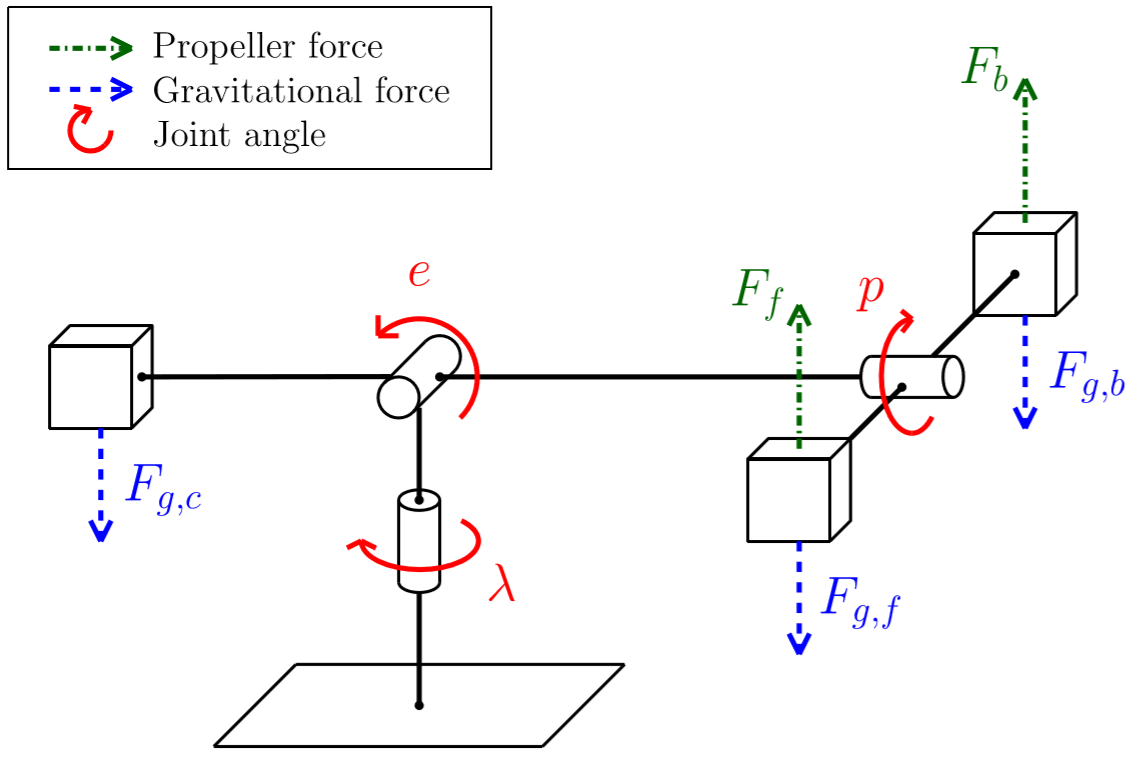
\includegraphics[scale=0.5]{fig/heli_fig_1.png}
    \caption{Figure of helicopter forces}
    \label{fig:heli_1}
\end{figure}

Starting with Newton's second law of rotation for the three system states travel $\lambda$, pitch $p$ and elevation $e$, which states that the net external torque equals the product of the moment of inertia and the angular acceleration,
\begin{equation}
    \begin{split}
        J_{\lambda} \ddot{\lambda} &= \sum{\tau_{\lambda}} \\
        J_p \ddot{p} &= \sum{\tau_p} \\
        J_e \ddot{e} &= \sum{\tau_e} \: \: .
    \end{split}
\end{equation}

Note that all friction, both aerodynamic drag and friction in the joints is neglected.

It is assumed that the the forces generated by the propellers is proportional to the voltages applied,
\begin{equation}
    \begin{split}
        F_f = K_f V_f \: \: ,\\
        F_b = K_b V_b \: \: ,
        \end{split}
\end{equation}
where $K_f$and $K_b$ are the proportionality constants.

Starting with the travel $\lambda$, the net external torque will  
\begin{equation}
    J_{\lambda} \ddot{\lambda} = (V_b - V_f) l_h \cos{e} \sin{p} \: \: .
\end{equation}

For the pitch $p$, the contributions are the propellers force, such that 
\begin{equation}
    J_{p} \ddot{p} = F_f l_p  - F_b l_p  \: \: .
\end{equation}

For elevation $e$, the contributions are the propellers affected by the angle of the pitch as well as the weight of both arms, such that 
\begin{equation}
    J_{e} \ddot{e} = (F_f + F_b)l_h \cos{p} -2 m_p g l_h  \cos{e} + m_c g l_c \cos{e}  \: \: .
\end{equation}
Denoting the voltage difference $V_f - V_b$ as $V_d$, and the voltage sum $V_f + V_b$ as $V_s$ in addition to defining the following constants,
\begin{equation}
    \begin{split}
        L_1 &= K_f l_p \: \: , \\ 
        L_2 &= g(m_c l_c  - 2 m_p l_h) \: \: , \\
        L_3 &= K_f l_h \: \: ,\\ 
    \end{split}
\end{equation}
the following system equations are presented,
\begin{equation}\label{eq:nonlin_heli}
    \begin{split}
        J_{\lambda} \ddot{\lambda} &= -L_3 V_s \cos{e} \sin{p} \: \: ,\\ 
        J_p \ddot{p} &= L_1 V_d \: \: ,\\ 
        J_e \ddot{e} &= L_2 \cos{e} + L_3 V_s \cos{p} \: \: .\\ 
    \end{split}
\end{equation}

Since \acrshort{mpc} solves a \acrshort{qp}-problem at every time step, the system equations in \eqref{eq:nonlin_heli} will be  linearized around the helicopters equilibrium point. This calculation is described in appendix \ref{ch:linear_heli_model}.

The resulting first-order discrete linear time system is 

\begin{equation}
    \begin{split}
        x^+ &= Ax + Bu \: , \: \: \\
        A &= \m{1 & h & 0 & 0 & 0 & 0 \\
                0 & 1 & -hK_2 & 0 & 0 & 0 \\
                0 & 0 & 1 & h & 0 & 0 \\
                0 & 0 & -hK_1 K_{pp} & 1-hK_1 K_{pd} & 0 & 0 \\
                0 & 0 & 0 & 0 & 1 & h \\
                0 & 0 & 0 & 0 & -hK_3 K_{ep} & 1-hK_3 K_{ed}}, \\
        B &= \m{0 & 0 \\ 0 & 0 \\ 0 & 0 \\
                h K_1 K_{pp} & 0 \\ 0 & 0 \\ 0 & h K_3 K_{ep}} \: \: ,
    \end{split}
\end{equation}
with $x = \m{\lambda & \dot{\lambda} & p & \dot p & e & \dot e }^\top$, $u = \m{p_c & e_c}^\top$.



\section{Modelling constant disturbance} \label{sec:estimator}

As described above, the offset described is a constant drift in the travel, so
\begin{equation}
    A_d = \m{1 \\ 0 \\ 0 \\ 0 \\ 0 \\ 0 }^\top \: \: . 
\end{equation}

The implementation of the state estimator and the modelling of the constant disturbance seems simple enough. 


The results of how the estimator performs is presented in section \ref{sec:results}, Results. 

\subsection{Choosing poles for estimator gain $L$}

The strategy for choosing poles in discrete time is choosing them in a continual time space and then transforming them to poles in the discrete time space using the equation,
\begin{equation}
    z = e^{h \cdot p} \: \: ,
\end{equation}
where p is the pole in the continual time space, h is the sampling frequency, and z is the new pole in the discrete time space. 

Legg til figure

When selecting poles for state observers, it is important that the slowest eigenvalue of $A-LC$ is "faster", i.e. more negative than all the eigenvalues of $A - BK$. The placement of the poles in the left half plane also determine the step response of the error dynamics of the observer, however this is not as important, as long as the step response is stable and approaches zero faster than the state dynamics $A - BK$. 

The poles chosen for calculating the estimator gain where
\begin{equation}
    \begin{split}
        p = \m{0.3 \\ 0.4 \\ 0.5 \pm 0.15 i \\ 0.52 \pm 0.05 i \\ 0.6} \: \: .
    \end{split}
\end{equation}

Using the MATLAB function \verb|place(A,B,eig||, which calculates the matrix $K$ such that $A - BK$ has the eigenvalues given in $eig$. For the estimator gain, the code used was:
\begin{lstlisting}
L = place(system.A', system.C', p];
\end{lstlisting}

This because to use the place function for $A - BK$, where $A$ and $B$ are inputs, the symmetric system matrix for the observer $A_L = A - LC$ = $A_L^\top = A^\top - C^\top L^\top$.

The \textit{principle of separation of estimation and control} states that choice of observer gain $L$ and the choice of state feedback $K$ are independent of one another. This can be shown easily by looking at the complete system model
\begin{equation}
    \m{x^+ \\ e^+} = \m{A-BK & BK \\ 0 & A-LC} \m{x \\ e} \: \: .
\end{equation}
Since this is an upper triangular matrix, the eigenvalues of the system are just the eigenvalues of $A - BK$ and $A - LC$
%\cite{https://math.stackexchange.com/questions/21454/prove-that-the-eigenvalues-of-a-block-matrix-are-the-combined-eigenvalues-of-its}.
The stability of these two states are not dependent on each other
%\cite{https://en.wikipedia.org/wiki/Separation_principle}.


\section{Selection of constraints}

The only hard constraints on the states are there to reflect the limitations of the actual system. The pitch angel is limited, because this axis on the helicopter does not go all the way around. The elevation is also limited, mostly due to the table. 

One of the hard constraints on the travel, $\lambda$, is there to ensure feasibility. As mentioned in section \ref{sec:terminal_constraint}, starting too far away from the equilibrium point results in infeasibility, because of the terminal constraint. Therefore a hard constraint on $\lambda$ is only there to avoid infeasibility during run-time. 


The soft constraint $-30 deg - \epsilon_p \leq p \leq 30 deg + \epsilon_p$ is added, where $\epsilon_p \geq 0$ is also an optimization variable. This is so the linearized model will stay accurate, because $\sin p \approx p$ for small values of p.

PLOT

